\documentclass[parskip=full,11pt]{scrartcl}
%\usepackage{pdfpages}
\usepackage[utf8]{inputenc}
\usepackage{amssymb}
\usepackage[T1]{fontenc}
\usepackage[german]{babel}
\usepackage[yyyymmdd]{datetime} 
\usepackage{hyperref}
\usepackage[toc, nonumberlist, automake]{glossaries} %added automake option
\usepackage{csquotes}
\usepackage{graphicx}
\hypersetup{
 		pdftitle={Entwurf},
 		bookmarks=true,
 }
\usepackage{fancyhdr}%<-------------to control headers and footers
\usepackage[a4paper,margin=1in,footskip=.25in]{geometry}
\fancyhf{}
\fancyfoot[C]{\thepage} %<----to get page number below text
\pagestyle{fancy} %<-------the page style itself
 
\title{Entwurf}
\subtitle{Autorisierungsmanagement für eine virtuelle Forschungsumgebung für Geodaten}
\author{Alex\\Anastasia\\Atanas\\Dannie\\ Houra\\Sonya\\}
\date{11.01.18}
 % define custom lists
\usepackage{enumitem}

% add glossary
\makeglossaries
\newglossaryentry{GUI}
{
	name={GUI},
	description={Abk. GUI von englisch \textbf{G}raphical \textbf{U}ser \textbf{I}nterface,ist Grafische Benutzeroberfläche oder auch grafische Benutzerschnittstelle, über die eine Person eine Software kontrollieren kann.  Im Idealfall ist sie benutzerfreundlich, so dass die Interaktion auf natürliche und intuitive Weise geschehen kannIm Idealfall ist sie benutzerfreundlich, so dass die Interaktion auf natürliche und intuitive Weise geschehen kann}, 
}
\newglossaryentry{ORM}
{
	name={ORM},
	description={Abk. ORM von englisch \textbf{O}bject-\textbf{R}elational \textbf{M}apping, ist eine Programmiertechnik zum Konvertieren von Daten zwischen inkompatiblen Systemen mit objektorientierten Programmiersprachen. Dies erzeugt in Wirklichkeit eine "virtuelle Objektdatenbank", die innerhalb der Programmiersprache verwendet werden kann}, 
}
\newglossaryentry{HTML}
{
	name={HTML},
	description={Abk. HTML von englisch \textbf{H}yper\textbf{t}ext \textbf{M}arkup \textbf{L}anguage, Auf Deutsch bedeutet dies  „Auszeichnungssprache für verknüpften Text“. Er ist Voraussetzung für die Programmierung und das Design von Webinhalten. Andere Standards wie PHP bauen in erheblichem Maße auf HTML auf }, 
}
\newglossaryentry{URL}
{
	name={URL},
	description={Abk. URL von englisch \textbf{U}niform \textbf{R}esource \textbf{L}ocator, wird häufig als Webadresse bezeichnet. Diese Adresse wird verwendet, um eine im Web vorhandene Ressource durch eine ASCII-Zeichenfolge zu bezeichnen. Ressourcen können variiert werden (Webseite, Video, Ton, Bild, Animation, E-Mail-Adresse ...)}, 
}



\usepackage{linegoal,listings}
\newsavebox{\mylisting}
\makeatletter
\newcommand{\lstInline}[2][,]{%
	\begingroup%
	\lstset{#1}% Set any keys locally
	\begin{lrbox}{\mylisting}\lstinline!#2!\end{lrbox}% Store listing in \mylisting
	\setlength{\@tempdima}{\linegoal}% Space left on line.
	\ifdim\wd\mylisting>\@tempdima\hfill\\\fi% Insert line break
	\lstinline!#2!% Reset listing
	\endgroup%
}
\makeatother
\setlength{\parindent}{0pt}% Just for this example

\lstset{basicstyle=\footnotesize\ttfamily,breaklines=true}
\lstset{framextopmargin=50pt,frame=bottomline,showstringspaces=false,upquote=true}


\RedeclareSectionCommand[style=section,indent=0pt,font=\usekomafont{partnumber}]{part}
\renewcommand*{\partformat}{\thepart\enskip}

\RedeclareSectionCommand[beforeskip=0pt ,afterskip=0pt]{subparagraph}



\newcommand{\class}[1]{\subsubsection*{\lstinline[basicstyle=\ttfamily\large]{#1}}}

% command for an attribute
\newcommand{\atr}[4]{\lstinline{[#3]} \textbf{\lstinline{#1 : #2}} \newline #4}

% command for a method
\newcommand{\mtd}[5]{\lstinline{[#4]} \textbf{\lstinline{#1(#3) : #2}} \newline #5}

% command for a constructor
\newcommand{\ctr}[4]{\lstinline{[#3]} \textbf{\lstinline{#1(#2)}} \newline #4}
%command for formating an inline source code
\newcommand{\inlinecode}[1]{\lstInline[breaklines=true]{#1}}

% make the bullet symbol in lists a circle for level 2
\renewcommand{\labelitemii}{$\circ$}




 
\begin{document}
 
 \begin{titlepage}
 	
 	\begin{center}
 	
\includegraphics[width=0.5\linewidth]{res/KITLogo.png}\\
 	\vspace{2cm}
 	{\scshape\LARGE\bfseries Entwurf \par}
 	\vspace{0.5cm}
 	{\scshape\Large Praxis der Softwareentwicklung\\}
 	\vspace{1cm}
 	{\scshape\Large Wintersemester 17/18\\}
 	\vspace{2cm}
 	{\huge\bfseries Autorisierungsmanagement für eine virtuelle Forschungsumgebung für Geodaten\par}
 	\vspace{2cm}
 	\vfill
 	{\bfseries {\Large Autoren}:\par}
 	{\Large Bachvarov, Aleksandar }\\
 	{\Large Dimitrov, Atanas }\\
 	{\Large Mortazavi Moshkenan, Houraalsadat }\\
 	{\Large Sakly, Khalil }\\
 	{\Large Slobodyanik, Anastasia }\\
 	{\Large Voneva, Sonya}\\
 	\vfill
 	{\large 11.01.18 \par}
 	\end{center}
 \end{titlepage}
 
 \tableofcontents
 
 \newpage
 \section{Einleitung}
 
Während der Entwurfsphase wurde das Konzept für das zu erstellende Produkt formuliert. Die in diesem Dokument definierte Softwarearchitektur legt die Struktur und das Verhalten des Produkts fest. Durch Bestimmung grundlegender Entwurfsentscheidungen haben sich einige sinnvolle Änderungen zum Pflichtenheft ergeben. \\
Für die Funktion „Benutzer suchen“ wurden Suchparameter erweitert: die Suche soll anhand von Name, Email sowie Domain des Benutzers möglich sein. 
Nach dem Löschen einer Ressource werden alle Benutzer, die Besitzerrechte für diese Ressource hatten, benachrichtigt. 
Als Ressourcendaten werden auch Typ und kurze Beschreibung der Ressourcen gespeichert. 
Administratoren des Portals sollen in der Lage sein andere Benutzer zu blockieren.

 
 \section{Architektur}
 
 \subsection{Model View Template (MVT)} \label{MVT}
Beim Design des Autorisierungsmanagement Web-Portal wird schnell deutlich, dass eine strikte Trennung
zwischen Datenbank, Applikationslogik (Code) und Benutzeroberfläche (view) von Vorteil ist. Das Model-View-Template Prinzip (MVT),Das in Abbildung 1 gezeichnet ist, realisiert diese Trennung und wird in der Webanwendung eingesetzt.\\
Das Model-View-Template ist eine Ableitung des Architektur-Pattern-View-Presenter (MVP) -Musters und wird hauptsächlich zum Erstellen von Benutzerschnittstellen verwendet.\\
 
 
 \begin{figure}[ht!]
 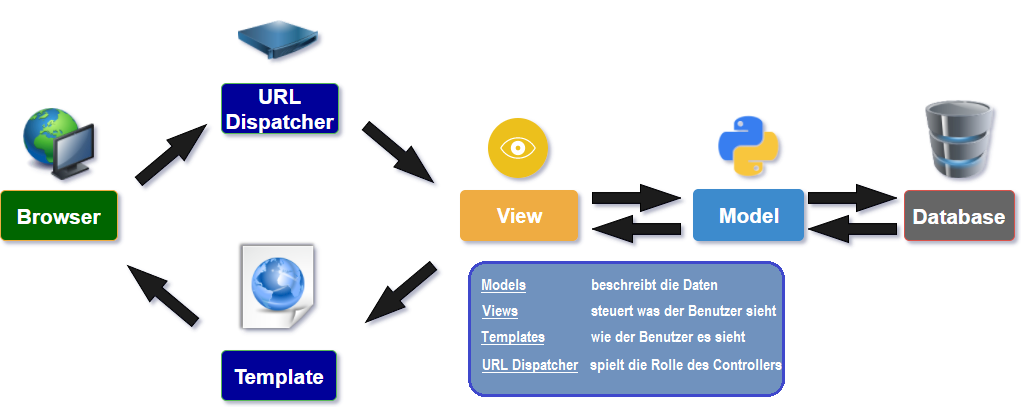
\includegraphics[width=1.1\textwidth]{res/MVTdiagramm.png}
  	 	\centering
  	    \caption{MVT Architektur}
 \end{figure}
  \newpage


 	\textbf{•} Der \textbf{URL-Dispatcher} \emph{(urls.py)} ordnet die angeforderte \gls{URL} einer \textbf{View-Funktion} zu und ruft sie auf.\\
 	\textbf{•} Die \textbf{View-Funktion} \emph{(views.py)} führt die angeforderte Aktion aus, bei der normalerweise in die Datenbank gelesen oder geschrieben wird. es kann auch andere Aufgaben beinhalten.\\
 	\textbf{•} Das \textbf{Model} \emph{(models.py)} definiert die Daten in Python und interagiert damit. Dies ist normalerweise in einer relationalen Datenbank \emph{(SQLite)} enthalten.\\
 	\textbf{•} Nach der Ausführung der angeforderten Aufgaben gibt die \textbf{View} ein HTTP-Antwortobjekt an den Webbrowser zurück, normalerweise nach dem Übergeben der Daten durch ein \textbf{Template}.\\
 	\textbf{•} \textbf{Template} gibt normalerweise \gls{HTML}-Seiten zurück. Die Django-Template-sprache bietet HTML-Autoren eine einfach zu erlernende Syntax und bietet gleichzeitig die gesamte für die Präsentationslogik erforderliche Leistung. \\
 	

 \subsection{Betrieb des Django ORM} 
 
Das \gls{ORM} Django ist ein in Python geschriebenes quelloffenes Webframework, das Beispielweise folgendermaßen funktioniert :\\
 • Erstellt Django SQL-Tabellen aus der Modellen (klassen) mit alle klassen-Attributen als Tabellenspalten, z.b SQL-Tabelle 'Request' aus dem Modell 'Request'. All dies geschieht wiederum ohne eine SQL-Abfrage zu schreiben.\\
 • Um die Tabellen auszufüllen wird die Methode save() benutzt.\\
 • Auf die gleiche Weise ist es möglich, alle Einträge der Tabelle zu erhalten ,Daher werden Instanzen von dem gewünschten Objekt zurückgegeben, einen für jeden Eintrag in der Tabelle, ein Beispiel für alle Request-Objekte zu haben wird in der Abbildung 2 gezeigt:\\

  	\vspace{2cm}



\begin{figure}[ht!]
  	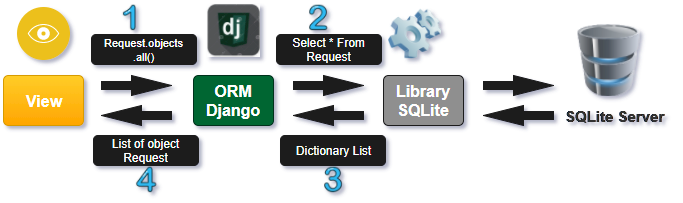
\includegraphics[width=1.05\textwidth]{res/MVTpart2.png}
  	 	\centering
  	    \caption{MVT mit Django}
 \end{figure}

 	


 \subsection{Paketstruktur}%oder Paketen?
 
 \subsection{Entwurfsmuster}
 Bei diesem Entwurf werden Entwurfsmuster verwendet, um einzelne Komponenten voneinander zu entkoppeln und das Geheimnisprinzip zu unterstützen. 
 \subsubsection*{MVT-Muster} 
 Bei diesem Entwurf wird das  \hyperref[MVT]{Model-View-Template} Architekturmuster verwendet.
 \subsubsection*{Strategie-Muster}
 \begin{figure}[ht!]
 	\centering
 	\includegraphics[width=\textwidth]{res/strategie.png}
 	\caption{Sterategie-Muster}
 \end{figure}
 Das Strategy-Muster kommt in den Klassen ``\textit{Reauest}``, ``\textit{AccessRequest}`` und ``\textit{DeletionRequest}`` bei der Funktion ``\textit{accept()}`` zum Einsatz. Dieses Muster hat das Ziel, eine Familie von Algorithmen zu definieren, zu kapseln und austauschbar zu machen.
 
 \subsubsection*{Befehlsmuster}
 \begin{figure}[ht!]
 	\centering
 	\includegraphics[width=\textwidth]{res/Befehl.png}
 	\caption{Befehlsmuster}
 	\label{Befehl}
 \end{figure}
 Das Befehlsmuster ist zur Bearbeitung von den Requests (Funktionen ``\textit{deny()}`` und ``\textit{accept()}`` in Klasse ``\textit{Reauest}``) verwendet.Mit Hilfe dieses Musters wird die Bearbeitung der Requests von den Requests selbst, wie in der   \hyperref[Befehl]{Abbildung 4} angezeigt ist, getrennt.\\
Das Befehlsmusters ermöglicht es, ein bestimmtes Ereignis in einem dafür vorgesehenen Handler
zu bearbeiten und dieses damit in einem Objekt zu kapseln. Jeder Handler lässt sich eindeutig einer Aufgabe
und einem Ereignis zuordnen, sodass keine Verschränkung zwischen zwei verschiedenen Handlern auftritt.
Außerdem lässt sich leichter ein weiterer Handler hinzufügen oder ein bestehender Handler austauschen.
 
 \subsubsection*{Bequemlichkeitsmethode-Muster}
 Das Bequemlichkeitsmethode-Muster ist in der Klasse ``\textit{Owner}``
 bei den Funktionen ``\textit{allowAccessPermission(reqestID)}`` und ``\textit{allowAccessPermission(resourceID, userID)}`` verwendet.Dieses Muster dient zum Vereinfachen des Funktionenaufrufs durch die Bereitstellung häufig
genutzter Parameterkombinationen in zusätzlichen Funktionen
(Überladen).
  \subsection{URL Verzeichnis}
Alle Interaktionen zwischen den Benutzern und dem Produkt werden durch eine graphische Benutzeroberfläche (GUI) unterstützt. Die \gls{GUI} des Produkts wird als eine Webseite dargestellt, wobei sämtlicher Inhalt und Funktionalität unter URL Verzeichnis abgelegt werden (\hyperref[URL Struktur]{\mbox{Abbildung 5}}). 

\begin{figure}[ht!]
 	\centering
 	\includegraphics[width=\textwidth]{res/urls_Diagram.png}
 	\caption{URL Struktur}
 	\label{URL-Struktur}
 \end{figure}
 
\textbf{pse-authoritation.com} – Mockup-Seite, dient zum Einloggen in das Portal, enthält Autorisierungsformular und wird nach der Entwicklung durch Autorisierungsmanagement des Systems, in welches das Projekt integriert wird, ersetzt. 
 
\renewcommand{\labelitemi}{$\bullet$}
\renewcommand{\labelitemii}{$\bullet$}
\renewcommand{\labelitemiii}{$\bullet$}
\begin{itemize}[itemsep=0pt]
\item \textbf{/profil} - Benutzerprofil-Seite, enthält persönliche Information des Benutzers und Übersicht der Requeste, die an den Benutzer adressiert sind.\\

Benutzerprofil-Seite ist mit Subseiten versehen:
\begin{itemize}[itemsep=0pt]
\item \textbf{/handle{\_}request{\_}$<$requestID$>$} - Dialog für Bearbeitung des Requests, enthält ``Annehmen''- und ``Ablehnen``-Buttons, sowie ein Eingabefeld für kurze Begründung.
\item \textbf{/resources} - Seite mit Übersicht von Ressourcen, für die der Benutzer Besitzerrechte hat. Diese Seite enthält Subseiten:
\begin{itemize}[itemsep=0pt]
\item \textbf{/add{\_}new{\_}resource} - Seite für Erstellen neuer Ressourcen. Enthält Upload-Dialog, Dialog für Vergabe von Rechten und Eingabefelder für Namen und Beschreibung der Ressourcen.
\item \textbf{/$<$resourceID$>${\_}edit{\_}users{\_}permissions} - Seite für Vergabe und Entzug von Rechten für die Ressource.
\item \textbf{/$<$resourceID$>${\_}send{\_}deletion{\_}request} - Dialog für Absenden von Löschrequest für die Ressource.
\end{itemize}
\end{itemize}


\item \textbf{/manage{\_}users} - Administratorseite für Benutzerverwaltung, enthält Liste von Benutzern und Subseiten:
\begin{itemize}[itemsep=0pt]
\item \textbf{/block{\_}user} - Dialog zum Blockieren des Users.
\item \textbf{/delete{\_}user} - Dialog zum Löschen des Users.
\item \textbf{/$<$userID$>${\_}permissions{\_}for{\_}resources} - Dialog zur Änderung von Rechten des Benutzers.
\end{itemize}

\item \textbf{/manage{\_}resources} - Administratorseite für Ressourcenverwaltung, enthält Liste von Ressourcen und Subseiten:
\begin{itemize}[itemsep=0pt]
\item \textbf{/$<$resourceID$>${\_}permissions{\_}for{\_}users} - Dialog zur Änderung von Zugriffsrechten für die Ressource. 
\item \textbf{/delete{\_}resource} - Dialog zum Löschen der Ressource.
\end{itemize}
\item \textbf{/resources{\_}owerview} - Übersicht von Ressourcen, enthält Liste aller Ressourcen und folgende Subseiten:
\begin{itemize}[itemsep=0pt]
\item \textbf{/$<$resourceID$>${\_}info} - enthält Metadaten der Ressource.
\item \textbf{/$<$resourceID$>${\_}send{\_}request} - Dialog zum Absenden des Requests für die Ressource.
\end{itemize}
\item \textbf{/<resourceID>} - Ressourcenseite, enthält Metadaten und Link für Zugriff auf die Ressource.
\end{itemize} 

 
 
 \section{Datenhaltung}
 
Relevante Daten über die Benutzer, Ressourcen, deren Beziehungen (Rechte) und Interaktionen (Requests) werden in einer Datenbank gespeichert. Das in diesem Projekt benutzte Framework Django bietet integrierte  objektrelationale Abbildung für die Datenbanksysteme MySQL, Oracle, PostgreSQL und SQLite.\\
Da SQLite-Bibliotheken sich direkt in Anwendungen integrieren lassen, sodass keine weitere Server-Software benötigt wird, wurde entschieden, SQLite3-Syntax zu verwenden. Im Projekt wird das eingebettete Datenbanksystem (für Frontend nicht sichtbar) entworfen, sodass auf erweiterte Funktionalitäten von komplizierteren Datenbanksysteme verzichtet werden kann. Dabei entstehen auch einige Vorteile: die SQLite-Bibliothek ist nur wenige hundert Kilobyte groß und durch das Einbinden der Bibliothek wird die Anwendung um Datenbankfunktionen erweitert, ohne auf externe Softwarepakete angewiesen zu sein.
 \subsection{Datenbank}
 \begin{figure}[ht!]
 	\centering
 	\includegraphics[width=0.75\textwidth]{res/database.png}
 	\caption{Datenbankschema}
 \end{figure}
 \newpage
 
    \begin{center}
    \textit{``A model is the single, definitive source of information about your data. It contains the essential fields and behaviors of the data you’re storing. Generally, each model maps to a single database table.``}
    \end{center}
    —Models | Django documentation\\\\
    
Die Tabelle ``User`` speichert einen eindeutigen Identifikator (\textit{ID}) des Benutzers, seinen Vor- und Nachnamen, sowie das Datum, an dem er sich registriert hat. Zusätzlich hat die Tabelle eine Spalte ``is\char`_admin``, die zur Unterscheidung zwischen ``normalem`` Benutzer und Administrator dient.\\
Metadaten über die Ressourcen werden in der Tabelle ``Resource`` gespeichert: ID, Name, generischer Typ, kurze Beschreibung und Erstellungsdatum.\\
In der Tabelle "Request" werden relevante Daten über die Requests gespeichert: ID, Erstellungsdatum, Typ des Requests (Zugriffs- oder Löschrequest), ID der Ressource, für die der Request gesendet wird und ID des Absenders. Requests werden sofort nach der Erstellung gespeichert und nach der Bearbeitung wieder gelöscht.\\
Abgesendete, noch nicht bearbeitete Requests werden in der Tabelle ``ReceivedRequest`` dupliziert, dabei wird ein Eintrag pro Empfänger erstellt. Diese Tabelle enthält folgende Spalten: ID und Typ des Requests und ID des Empfängers.\\
Rechte werden in der Tabelle ``Permission`` dargestellt. Jeder Eintrag dieser Tabelle präsentiert entweder ein Zugriffs- oder Besitzerrechte, dabei werden folgende Attribute gespeichert: ID des Benutzers, ID der Ressource und Typ des Eintrags (Zugriffs- oder Besitzerrechte).
   \\
 
 \subsection{Logging}
 Mithilfe von einem externen Django Module (``Logging``) wird eine Log-Datei geführt. Diese Datei beinhaltet zeitlichgeordnete Ereignisse vom System. Informationen wie Senden eines Requests, Bearbeitung eines Requests, Erstellen/Löschen einer Ressource und Editieren von Rechten können der Log-Datei entnommen werden. Zu jedem Ereignis wird auch den genauen Zeitpunkt gespeichert.
 
 
 \section{Paketenübersicht}
 
 
 \section{Klassenübersicht}
 \subsection{Model}
 \paragraph*{Klasse User}
 User-Klasse bildet eine Elternklasse aller Benutzertypen. Sie stellt alle Attribute fest, die für Abstraktion des Benutzers notwendig sind, und beschreibt Aktivitäten, die von allen Benutzertypen ausgeführt werden können.
\paragraph*{Attribute} % skip this if there are no attribute
\begin{itemize}
	\item \atr{name}{String}{private}{
	bla 
	}
\end{itemize}
\subparagraph*{Methoden}  % skip this if there are no methods
\begin{itemize}
	\item \mtd{foo}{String}{a:String}{public}{
	bla  \inlinecode{USER_ID}
	}
\end{itemize}
  \paragraph*{Klasse Owner}
 \class{Owner extends User}
 bla bla
 
 \subparagraph*{Konstruktoren} % skip this if there are no constructors
\begin{itemize}
	\item \ctr{User}{a:String}{public}{
	bla
	}
\end{itemize}
\paragraph*{Attribute} % skip this if there are no attribute
\begin{itemize}
	\item \atr{name}{String}{private}{
	bla 
	}
\end{itemize}
\subparagraph*{Methoden}  % skip this if there are no methods
\begin{itemize}
	\item \mtd{foo}{String}{a:String}{public}{
	bla  \inlinecode{USER_ID}
	}
\end{itemize}
\subsection{View} 
 \section{Sonstige Diagrammen}
 \subsection{Zugriffsrequest schicken}
 \begin{figure}[ht!]
 	\centering
 	\includegraphics[width=\textwidth]{res/sendAccessRequest.png}
 	\caption{Zugriggsrequest schicken}
 	\label{fig:sendAccReq}
 \end{figure}
 
Von irgeneiner Viewklasse wird die Methode \enquote{sendAccessRequest(resourceID )} auf dem Benutzer \enquote{a}  aufgerufen. Erstens wird eine AccesRequest Instanz \enquote{b} erstellt und in der Datenbank gespeichert. Danach wird die Ressource, für den das Request geschickt wurde, von der Datenbank geholt und in der Variable \enquote{r} gespeichert. Auf der Ressourceninstanz \enquote{r} wird dann getOwners() aufgerufen, was alle Besitzer des Ressource liefert. Auf allen Instanzen von diesen Besitzer(auf dem Diagramm als die Variable \enquote{list} bezeichnet) wird die Methode  \enquote{addAccessRequest(request)} aufgerufen. Das fügt den Request in der Liste der bekommenen, aber noch nicht bearbeiteten Requesten, hinzu. Eine passende Lognachricht (die in dem Diagramm gegebene ist nur als Beispiel gegeben, die echte Nachricht wird anders sein) wird in der Logdatei durch die Methode \enquote{info()} gespeichert. Danach wird eine Instanz der Djangoklasse \enquote{Emailmessage} erstellt. Als Parameter ist die Variable \enquote{list} gegeben. Damit ist gemeint, dass die Klasse alle Emails von den Besitzern in List nimmt. Der Konstruktor der Klasse nimmt auch andere Parameter als Emailnachricht, Sender usw, die im Diagramm nicht bezeichnet sind. Nach dem erfolgreichten Schicken der Emails mit der Methode  \enquote{send()} wird eine Lognachricht dafür in der Logdatei gespeichert. 
 
  \newpage
 \subsection{Zugriffsrequest genehmigen}
 \begin{figure}[ht!]
 	\centering
 	\includegraphics[width=\textwidth]{res/allowAccessPermission.png}
 	\caption{Zugriffsrequest genehmigen}
 \end{figure}
 
 Von irgeneiner Viewklasse wird die Methode \enquote{sendAccessRequest(resourceID )} auf dem Besitzer \enquote{a}  aufgerufen. Danach wird der Request von der Datenbank geholt in in der Variable \enquote{req} gespeichert. Danach wird auf \enquote{req} getSender aufgerufen und das Ergebnis(der Benutzer, der das Request geschickt hat) wird dann in \enquote{u} gespeichet. Das Gleiche passiert für das durch den Request angefragte Ressource durch die Methode \enquote{getResource()}. Auf \enquote{u} wird dann \enquote{addAccessPermission(resource)} aufgerufen, was intern der Benutzer \enquote{u} in der Liste \enquote{accessPermission} von Ressource hinzufügt. Eine Lognachricht wird in der Logdatei gespeichert. Die Methode \enquote{delete(requestID)} löscht den Request von der Datenbank. Von hier an ist das Diegramm ähnlich bis gleich zum Ende des Diegramms \hyperref[fig:sendAccReq]{Zugriffsrequest schicken}. 
 
  \newpage
 \subsection{Ressource erstellen}
 \begin{figure}[ht!]
 	\centering
 	\includegraphics[width=\textwidth]{res/Add_resourceDiagram.png}
 	\caption{Ressource erstellen}
 \end{figure}
 
Von irgeneiner Viewklasse wird die Methode \enquote{addResource()} auf dem Benutzer \enquote{a}  aufgerufen.\\ Erstens wird eine Resource Instanz \enquote{r} erstellt und in der Datenbank gespeichert.\\ Dann wird das Benutzer \enquote{a} zuerst als einer des Besitzers diese Resource \enquote{r} hinzugefügt durch seinen \enquote{UserID} mit Aufruf der Methode \enquote{addOwner(a.getUserID)}, danach als einer des Lesers diese Resource \enquote{r} durch seinen \enquote{UserID} mit Aufruf der Methode \enquote{addReader(a.getUserID)} .\\Am Ende wird eine Lognachricht über diesen ganzen Prozess  in der Logdatei gespeichert.

 
 
  \newpage
 \subsection{Ressource loeschen}
 \begin{figure}[ht!]
 	\centering
 	\includegraphics[width=\textwidth]{res/remove_resourceDiagram.png}
 	\caption{Ressource loeschen}
 \end{figure}
 
 
 Von der Viewklasse Manage-Resource wird die Methode \enquote{deleteResource()} auf dem Admin \enquote{a}  aufgerufen.\\ Erstens wird die Liste der \enquote{Owner} dieser Ressource vom Datenbank gelöscht, mit Aufruf der Methode \enquote{removeOwnerPermission.all()}, danach die Liste des Lesers diese Resource \ mit Aufruf der Methode \enquote{removeReaderPermission.all()}.\\
 Wenn die zwei Listen vom datenbank gelöscht sind dann wird die Ressource \enquote{r} auch gelöscht , mit hilfe der Methode \enquote{delete()}.\\ Am Ende wird eine Lognachricht über diesen ganzen Prozess  in der Logdatei gespeichert.\\
 
 
 \newpage
\setglossarystyle{altlist}
\printglossary	
	
 \end{document}
\grid
